\documentclass[12pt,a4paper]{report}

\usepackage[utf8]{inputenc}
\usepackage{amsmath}
\usepackage{amsfonts}
\usepackage{amssymb}
\usepackage{hyperref}
\usepackage{graphicx}
\usepackage{lscape}
\usepackage[francais]{babel}
\usepackage[left=2cm,right=2cm,top=2cm,bottom=2cm]{geometry}

\title{PJE\\\#Currentmood}
\author{Quentin Van de Kadsye \and Jérôme Tanghe}

\setlength{\parskip}{\baselineskip}

\begin{document}
\maketitle

\tableofcontents

% -----------------------------------------------------------------------------

\chapter{Le projet}

Il est parfois intéressant pour les entreprises de connaître l'humeur générale
des gens concernant un sujet donné. Twitter étant une plateforme où l'on peut
s'exprimer librement, c'est donc un emplacement de choix pour récolter ce type
d'information. Se pose alors le problème suivant : comment connaître rapidement
l'humeur des personnes sur un sujet donné?

\textbf{\#Currentmood} est un programme tentant de répondre à ce besoin. Écrit
en Java, il permet d'estimer l'humeur d'un ou plusieurs messages publiés sur
Twitter (\textit{tweet}), à l'aide d'une des trois méthodes proposées:

\begin{itemize}
    \item
        \textbf{Mots-clés:} utilise une liste de mots prédéfinis dans des
        fichiers pour déterminer l'humeur du tweet.
    \item
        \textbf{KNN:} évalue l'humeur d'un tweet en fonction de l'humeur de $k$
        autres tweets, en recherchant dans une base de données de tweets dont on
        connaît déjà l'humeur ceux qui contiennent les mêmes mots.
    \item
        \textbf{Classification bayésienne:} évalue la probabilité d'humeur d'un
        tweet en calculant la probabilité que les mots qu'il contient
        appartiennent à cette humeur à partir de la base de données.
\end{itemize}

% -----------------------------------------------------------------------------

\chapter{L'API Twitter}

Afin de communiquer avec Twitter, nous avons utilisé la librairie
\textbf{Twitter4J}\footnote{\href{http://twitter4j.org}{twitter4j.org}} qui
propose les fonctionnalités dont nous avons besoin pour mener à bien le projet.
Pour faciliter son implémentation, nous avons également créé une classe,
\texttt{CMTwitter}, s'interfaçant entre notre application et Twitter4J, comme le
montre la figure \ref{uml_cmtwitter} (page \pageref{uml_cmtwitter}).

\begin{landscape}
    \begin{figure}
        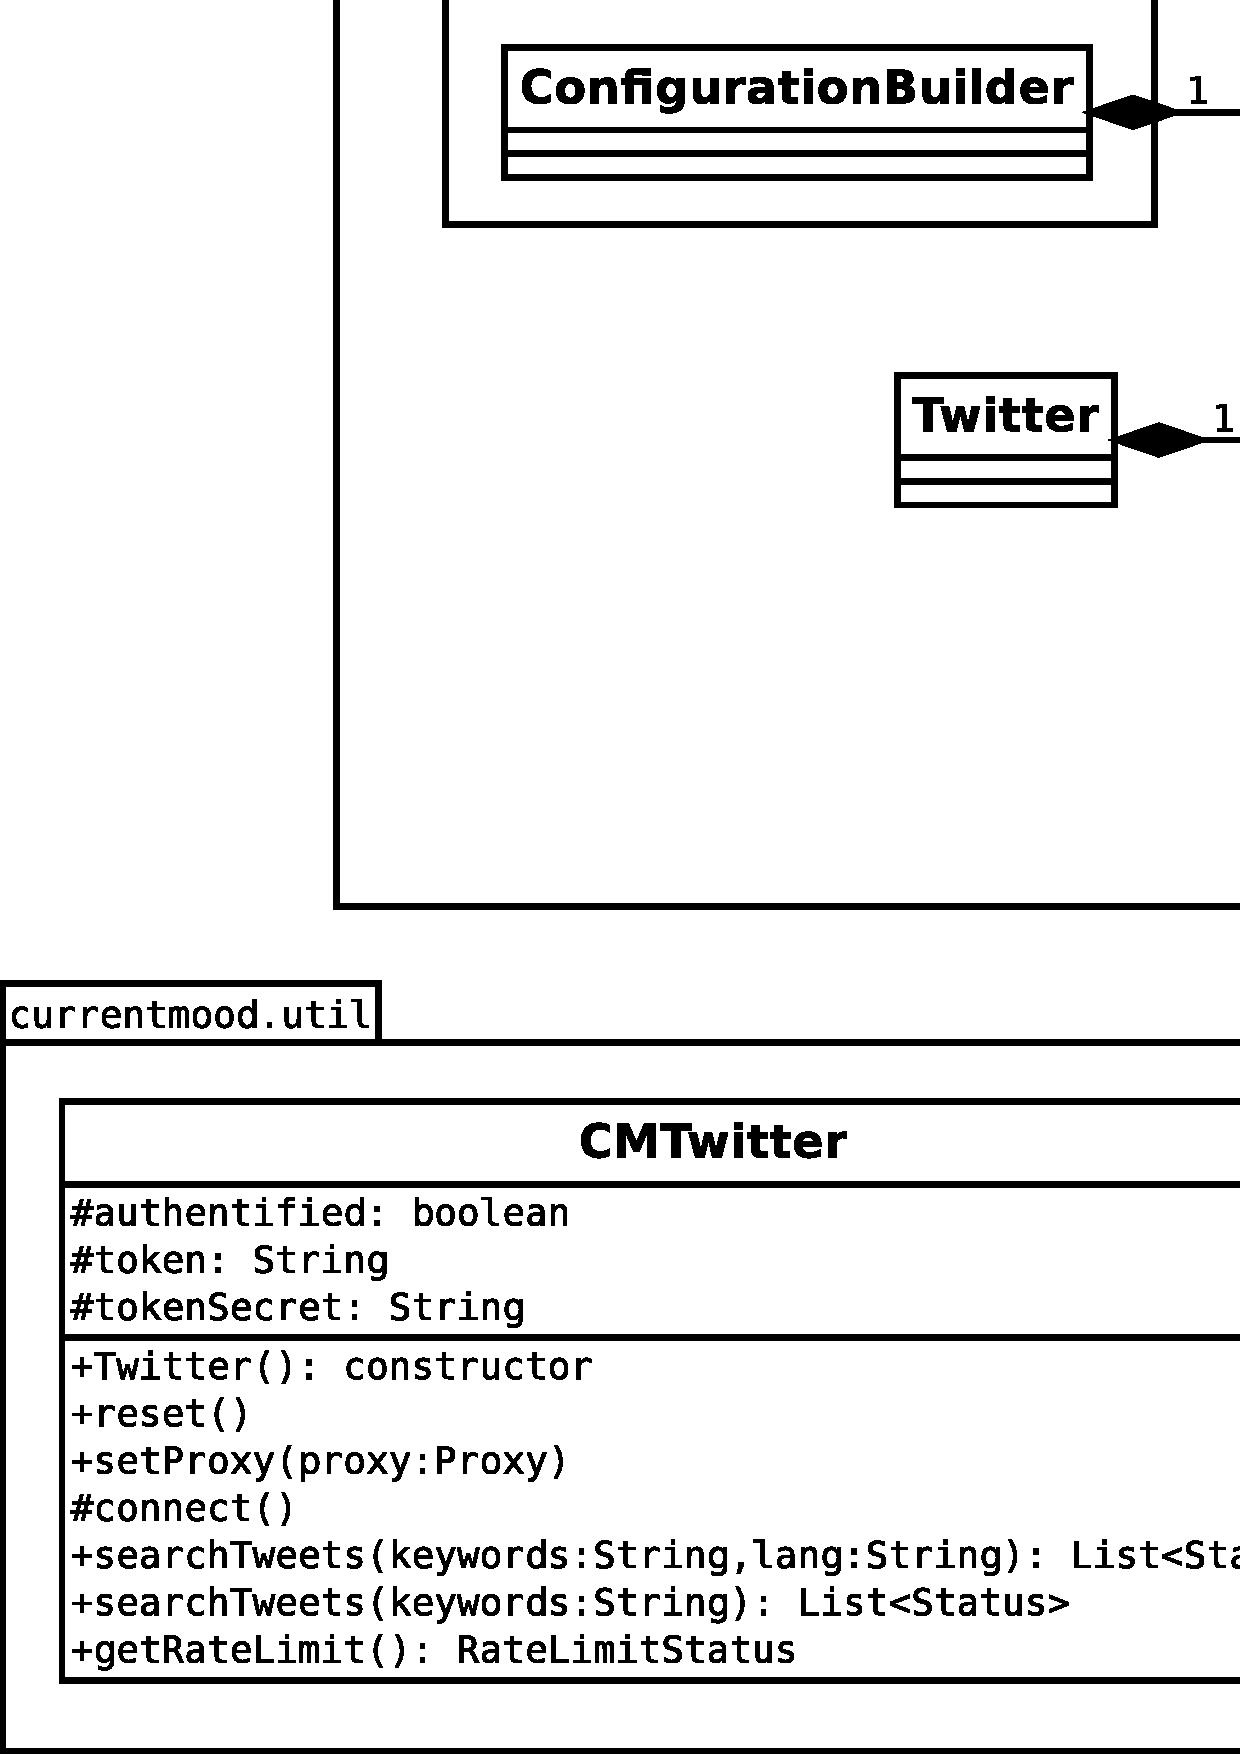
\includegraphics[width=25cm]{img/uml_cmtwitter.jpeg}
        \caption{Diagramme de classe montrant la classe \texttt{CMTwitter}
        permettant d'interfacer Twitter4J.}
        \label{uml_cmtwitter}
    \end{figure}
\end{landscape}

\end{document}
